\chapter{Theory}
In this chapter we explain the theoretical concepts relevant to this thesis. We start with explaining the physics behind our method in section \ref{bubble_physics}, in particular how bubbles interact with light. Next, we discuss the mathematical basics necessary for image processing such as Fourier theory and convolution in section \ref{image_processing}. Section \ref{machine_learning} explains the principle behind machine learning that our method relies on for classification. Finally, section \ref{the_object_detection_problem} formally introduces the object detection problem and our chosen criteria for evaluation. 

	\section{Bubble physics} \label{bubble_physics}
	
	\section{Image processing}	\label{image_processing}
	In the following we represent an image as a two dimensional signal written as a matrix \textit{\textbf{g}}. Therefore, $g_{m,n}$ denotes the pixel (i.e. picture element) at the \textit{m}-th row corresponding to the \textit{n}-th column. 
		\subsection{Fourier theory}
		The Fourier transform is an important image processing tool which is used to decompose an image into its since and cosine components. The output of the transformation represents the image in the Fourier or frequency domain, while the input image is the spacial domain. In the Fourier domain image, each point represents a particular frequency contained in the spatial domain image.
		The \textit{continuous} two-dimensional Fourier transform is defined as
		\begin{equation}
				\mathscr{F}\{ g(\mathbf{x})  \} = \hat{g}(\mathbf{k}) = 
				\int_{-\infty}^{\infty} g(\mathbf{x}) \text{exp}\left( -2 \pi \text{i} \mathbf{k}^T \mathbf{x}  \right) \text{d}\mathbf{x}
		\end{equation}
		and the inverse Fourier transform
		\begin{equation}
				\mathscr{F}^{-1}\{ \hat{g}(\mathbf{k}) \} = g(\mathbf{x}) =
				 \int_{-\infty}^{\infty} \hat{g}(\mathbf{k})
			\text{exp}\left( -2 \pi \text{i} \mathbf{k}^T \mathbf{x}  \right) \text{d}\mathbf{x}
		\end{equation}
		Where $\mathbf{x}$ and $\mathbf{k}$  are the two dimensional space and frequency vectors respectively. 
		
		Images however are discrete two dimensional signals, we therefore need to apply the \textit{Discrete} Fourier transform or DFT, defined as
		\begin{equation}
			\text{DFT}\{ g_{m,n} \} = \hat{g}_{u,v} = \dfrac{1}{MN} \sum_{m=0}^{M-1} \sum_{n=0}^{N-1}
			g_{m,n} \text{ exp} \left(  - \dfrac{2 \pi \text{i} m u}{M}  \right)
						\text{exp} \left(  - \dfrac{2 \pi \text{i} n u}{N}  \right)
		\end{equation}		 

		Similarly, the inverse 2-D DFT is defined as 
		
		\begin{equation}
		 \text{IDFT}\{\hat{g}_{u,v}\} = g_{m,n} = \sum_{m=0}^{M-1} \sum_{n=0}^{N-1} \hat{g}_{u,v}
			\text{ exp} \left(   \dfrac{2 \pi \text{i} m u}{M}  \right)
			\text{exp} \left(   \dfrac{2 \pi \text{i} n u}{N}  \right)
		\end{equation}
		
		
		\subsection{Convolution}
		Convolution is one of the most important operations in signal processing. Convolving two signals $g$ and $h$ produces a third signal that expresses how the shape of one is modified by the other. Formally, we define the continuous convolution as follows
		\begin{equation}
			(g \star h)(\mathbf{x}) = \int_{-\infty}^{\infty} 
			h(\mathbf{x}') g(\mathbf{x} - \mathbf{x}')
			\text{d}\mathbf{x}
		\end{equation}
		and the discrete two dimensional convolution as
		\begin{equation}
			g'_{m,n} = \sum_{m'=0}^{M-1} \sum_{n'=0}^{N-1}
			h_{m',n'} g_{m-m', n-n'}
		\end{equation}
		
		One important property of convolution is that we can express it as a multiplication in the Fourier domain. 
		\begin{equation}
		\mathscr{F}\{g \star h\} = N M \hat{h} \hat{g}
		\end{equation}
		This property, together with the fast Fourier implementation of the Fourier transform allows a fast computation of convolutions. 
		
		At the edge of the image, we typically extend the image with zero values (i.e. zero padding). This introduces an error when applying filters at the image border and we will mostly exclude the border when using filters (see chapter \ref{the_algorithm} for more details).
		
		\subsection{Smoothing}
		Smoothing an image means convolving an image with a smoothing filter. A smoothing or averaging filters must ideally fulfill following conditions
		\begin{enumerate}
			\item Zero-shift: $\Im (\hat{h}(\mathbf{k})) = 0$
			\item Preservation of mean value: $\hat{h}(0) = 1 $
			\item Monotonous decrease: $ \hat{h}(k_1) \leq \hat{h}(k_2) $ for $ k_2 > k_2 $
			\item Isotropy: $\hat{h}(\mathbf{k}) = \hat{h}(| \mathbf{k} |)$ \textcolor{red}{stimmt das ??}
		\end{enumerate}
		
		In this work, we will be using Gaussian filters for one and two dimensional smoothing. Although Gaussian filters are not ideal, e.g. isotropy is violated for small standard deviations, it is still a good approximation for an ideal low pass filter. Computing the Fourier transform (for convolution) is also faster for a Gaussian filter. The $m$-th component of a one dimensional Gaussian filter mask can be obtained from the Gaussian function
		\begin{equation}
		G_{m} = \dfrac{1}{2 \pi \sigma^2} \text{ exp}
			 \left( 
			 	- \dfrac{(m-\mu)^2}{2 \sigma^2}
			 \right)
		\end{equation}
		Where $\mu$ is the mean, i.e. Gaussian peak's position and $\sigma$ is the standard deviation, i.e. peak's width.
		
		Figure \ref{fig:gauss_intro} show a Gaussian curve in one and two dimensions as well as the result of convolving an image with a Gaussian filter mask. 
		\begin{figure}
		    \centering
		    \begin{subfigure}[b]{0.3\textwidth}
		        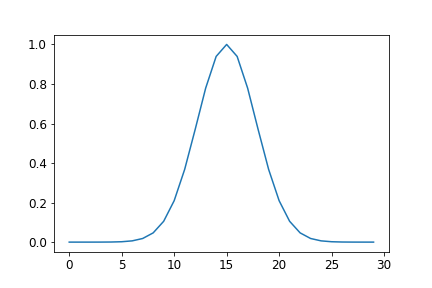
\includegraphics[width=\textwidth]{graphs/gauss_sigma_2.png}
		        \caption{1D Gaussian signal with $\mu=15$ and $\sigma=2$}
		    \end{subfigure}
		    
		    \begin{subfigure}[b]{0.3\textwidth}
		        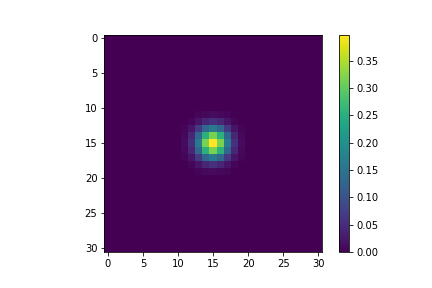
\includegraphics[width=\textwidth]{images/gauss_sigma_2.png}
		        \caption{2D Gaussian signal with $\mu_x = \mu_y = 15$ and $\sigma_x = \sigma_y = 2$}
		    \end{subfigure}
		    
		    \begin{subfigure}[b]{0.3\textwidth}
		        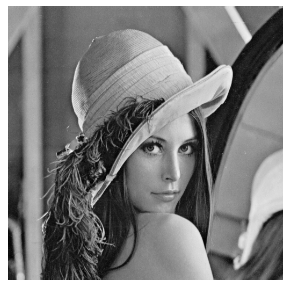
\includegraphics[width=\textwidth]{images/lena_orig.png}
		        \caption{Original image}
		    \end{subfigure}
		    ~ %add desired spacing between images, e. g. ~, \quad, \qquad, \hfill etc. 
		      %(or a blank line to force the subfigure onto a new line)
		    \begin{subfigure}[b]{0.3\textwidth}
		        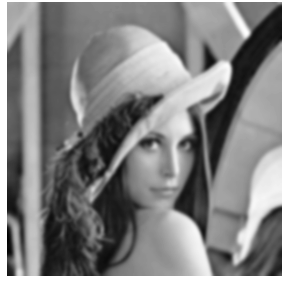
\includegraphics[width=\textwidth]{images/lena_smooth.png}
		        \caption{After convolution with 2D Gaussian mask}
		    \end{subfigure}
		    ~ %add desired spacing between images, e. g. ~, \quad, \qquad, \hfill etc. 
		    %(or a blank line to force the subfigure onto a new line)

		    \caption{Gaussian smoothing filter}
		    \label{fig:gauss_intro}
		\end{figure}


		\subsection{Derivation}
		\subsection{Orientation and Structure Tensor}
		
	
	\section{Machine Learning}
	\label{machine_learning}
	
	\section{The object detection problem}
	\label{the_object_detection_problem}
		\subsection{Evaluation Criteria}
